\documentclass{oblivoir}
\usepackage{graphicx}
\setcounter{section}{-1}

\usepackage{url}

\usepackage{xcolor}
\usepackage{listings}
%C스타일을 만들기위한 패키지


\definecolor{mGreen}{rgb}{0,0.6,0}
\definecolor{mGray}{rgb}{0.5,0.5,0.5}
\definecolor{mPurple}{rgb}{0.58,0,0.82}
\definecolor{backgroundColour}{rgb}{0.95,0.95,0.92}
%https://tex.stackexchange.com/questions/348651/c-code-to-add-in-the-document
\lstdefinestyle{CStyle}{
    backgroundcolor=\color{backgroundColour},   
    commentstyle=\color{mGreen},
    keywordstyle=\color{magenta},
    numberstyle=\tiny\color{mGray},
    stringstyle=\color{mPurple},
    basicstyle=\footnotesize,
    breakatwhitespace=false,         
    breaklines=true,                 
    captionpos=b,                    
    keepspaces=true,                 
    numbers=left,                    
    numbersep=5pt,                  
    showspaces=false,                
    showstringspaces=false,
    showtabs=false,                  
    tabsize=2,
    language=C
}


\begin{document}
    
    \tableofcontents
    \section{들어가며}

(원래 출판을 목적으로 썼던 책인데 출판사 사정으로 책 출판이 어려워져 인터넷에 그대로 공개합니다.)

\subsection{들어가며}

안녕하세요. 캐나다 렐릭 엔터테인먼트에서 시니어 그래픽 프로그래머로 일하고 있는 포프입니다. 이 쉐이더 입문 책은 제가 2007년 1월부터 2009년 12월까지 3년간 캐나다의 \href{https://www.artinstitutes.edu/}{The Art Institute of Vancouver} 대학에서 쉐이더 프로그래밍 강의를 하면서 축적한 자료와 지식을 글로 옮겨 놓은 것입니다.

\subsection{책을 쓰게 된 배경}

2007년에 제가 강의를 시작할 때, 수업시간에 사용할 교과서를 찾으려고 참 많은 노력을 했습니다. 하지만 시중에 나와있는 책들 중, 쉐이더 입문과목에 적합한 놈이 없더군요. (몇 년이 지난 지금에도 마찬가지인 것 같습니다.) 시중에 나와있는 쉐이더 책들은 대부분 이미 쉐이더 코드를 짤 줄 아는 중고급 프로그래머를 위한 것이었습니다. 따라서 쉐이더에 입문하는 학생들이 보면 뭔 소린지 몰라서 그냥 포기할 게 뻔했죠. 그나마 쉐이더 입문 내용이 DirectX 책에 담겨있는 경우가 있었지만 그 중에서도 마땅한 책이 없다고 생각했던 이유가
\begin{itemize}
    \item 쉐이더는 구색 맞추기 식으로 넣어놓아서 너무 수박 겉 핥기 식이다.
    \item 학계에 계신 분들이 쓴 책은 너무 이론이나 문법에만 치우쳐져 있다.
    \item 실무에 그다지 쓸모가 없는 내용들을 너무 많이 담고 있다.
    \item 지면수만 많아 책값이 너무 비싸다.
\end{itemize}


등 이었습니다. 그래서 결국엔 교과서 없이 강의를 시작했죠. 이론이나 수학에 치우치기 보다는 실무에 곧바로 쓸 수 있거나 실무에서 쓸 수 있는 기법의 기초가 되는 내용들만을 가르치는데 주력했습니다. 강의를 하면서 좋았던 점은 저는 그리 어렵지 않다고 생각해왔는데 학생들이 이해하지 못하는 부분들을 알아낼 수 있다는 거였죠. 그래서 그걸 다시 쉽게 이해시킬 수 있도록 강의자료를 다듬고 다듬은 결과가 바로 이 책입니다. 강의를 하는 3년 내내 게임프로그래밍 학과 학생들이 이 과목을 AI 대학의 가장 훌륭한 수업으로 꼽을 정도였으니 (좀 부끄럽지만) 이 책을 자신있게 권해드릴 수 있을 것 같습니다. 그리고 제 과목에서 만든 데모 프로그램을 포트폴리오로 삼아서 Ubisoft 및 EA같은 세계 유수의 회사에 취직한 학생들도 몇 됩니다. 가슴 뿌듯한 일이죠. ^^

현재는 게임개발에 좀 더 집중해 보려고 대학강의를 중단한 상황이지만 이 내용을 그냥 썩혀두기엔 아깝다고 생각되어 책을 내기로 결정을 했습니다. 이 책이 쉐이더를 배우시려는 분들에게 도움이 될 수 있었으면 좋겠습니다.

\subsection{이 책의 기본원칙}

강의에서도 그랬듯이 이 책을 쓸 때 다음의 원칙을 기초로 삼았습니다.

\begin{itemize}
    \item 실습 위주: 물론 쉐이더를 짤 때 수학이나 이론을 전혀 무시할 수는 없습니다. 하지만, 이론을 먼저 배우고 그걸 코드로 옮기는 것보단 일단 코드를 좀 짜본 뒤에 뭔가 막히면 이론을 찾아보는 것이 훨씬 훌륭한 학습방법입니다. 이렇게 문제를 해결하기 위해 찾아본 이론은 기억에 오래 남습니다. 따라서 이 책은 실습위주로 구성되어있습니다. 책의 내용을 한 줄씩 따라 하면서 코드를 짜다 보면 어느덧 배경 이론까지 적당히 이해하시게 될 겁니다.
    \item 쉬운 설명: 제 수업에 청강을 하러 오는 게임아트 학과 학생들도 꽤 있었습니다. 따라서 아티스트들도 이해할 수 있도록 쉽게 설명을 하는 것이 제 목표 중 하나였습니다. 그러려면 무언가를 설명할 때, 수학공식을 보여주기 보다는 실제 생활에서 일어나는 현상을 예로 드는 것이 낫더군요. 이 책을 쓸 때도 마찬가지 원칙을 따랐습니다. 책을 읽으시다 보면 100$\%$ 이론적으로 옳지 않은 설명들도 가끔 보실 겁니다. 이것은 말 그대로 설명을 쉽게 하기 위해 제가 이론들을 적당히 무시하였거나 아니면 저 조차 이론을 100$\%$ 제대로 이해하지 못하는 경우입니다. 게임 그래픽은 어차피 눈에 보이는 결과가 맞으면 그게 정답인 분야이므로 이론적으로 약간 틀려도 결과만 맞으면 전 크게 신경 쓰지 않습니다.
    \item 입문자만을 위한 책: 이 책은 순수하게 입문자를 위한 책입니다. 이미 고급기법을 다루는 훌륭한 책이 많이 나와있는 상황에서 굳이 그 책들과 경쟁할 필요를 못 느끼고, 중복되는 내용을 다루면서 지면수를 늘리고 싶지도 않기 때문입니다. 이 책을 보신 후에 쉐이더에 재미가 붙으신 분들이 다른 고급기법들을 즐겁게 찾아 보실 수 있다면 전 행복합니다. 그리고 정말 괜찮은 새 기법을 찾으시면 저에게 살짝 귀뜸이라도 해주시면 더 좋겠지요. ^^
    \item 순서대로 배우는 내용: 강의를 할 때 좋았던 점은 쉬운 내용부터 어려운 내용까지 순서대로 가르칠 수 있었다는 것입니다. 이 책도 그런 식으로 진행이 됩니다. 처음 장부터 시작해서 천천히 지식을 축적해간다고 할까요? 따라서 뒷장으로 가면 갈 수록 기본적인 내용은 다시 설명을 하지 않습니다. 예를 들면, 법선매핑을 배우기 전에 이미 조명기법들을 배워보므로 법선매핑에서는 조명기법에 대해 다시 설명하지 않는거죠. 따라서 이 책을 읽으실 때는 대학강의를 들으시듯이 처음부터 순서대로 읽으셔야 합니다. 이 책이 다른 쉐이더 책들처럼 여러 논문을 한군데 모아놓은 게 아니니 그 정도는 이해해주시면 좋겠습니다. 그리고 지면수도 그리 많지 않으니 무리한 요구는 아닐 거라고 믿습니다.
\end{itemize}


\subsection{이 책에서 다루는 내용}

이 책에서 다루는 내용은 정점쉐이더와 픽셀쉐이더를 이용한 쉐이더 기법들입니다. 이 책은 크게 세 부분으로 나뉘어져 있습니다.

\begin{itemize}
    \item 제1부: 쉐이더의 정의를 알아 본 뒤, 모든 쉐이더 기법의 기초가 되는 색상, 텍스처 매핑, 조명 쉐이더를 만들어 봅니다.
    \item 제2부: 1부에서 배운 내용에 살을 붙여 게임에서 널리 사용하는 스페큘러매핑, 법선매핑, 그림자 매핑 등의 기법들을 구현합니다.
    \item 제3부: 요즘 게임에서 점점 중요해져 가는 2D 이미지 처리 기법을 배워봅니다.
\end{itemize}


이 책에서 DirectX 10과 11에서 새로 추가된 지오메트리(geometry), 헐(hull), 연산(compute) 쉐이더들을 다루지 않는 이유는 초급자에겐 좀 어려운 내용일 뿐만 아니라 아직 실무에서 널리 이용되지 않기 때문입니다. 따라서 실용적인 내용을 알려드리기가 좀 어렵죠. DirectX 10이 처음 소개될 때만 해도 홍보자료에서는 엄청 대단한 것처럼 광고를 해댔지만 실제 실무에서 제대로 이용한 경우가 없으니까요. 일단 이 책에서 기초를 다잡으시면 몇 년 뒤에  이 내용을 배우셔도 크게 문제가 없을 겁니다.

\subsection{대상독자}

\textbf{프로그래머}

제가 가르쳤던 학생들은 게임 프로그래밍 학과 2학년 학생들이었습니다. 제 과목을 듣기 전에 C++, 3D 수학, DirectX 등을 이미 마친 학생들이었지요. 게임개발자 분들이 쉐이더 프로그래밍에 입문하는 과정도 이와 다르지 않다고 생각합니다. 최소한 DirectX는 마치신 뒤에 쉐이더를 살펴보시는 게 보통이니까요. 이 책의 대상독자도 마찬가지로 하겠습니다. 이 책을 보시려면 최소한 C++과 DirectX 정도는 공부하셨어야 합니다. 3D 수학까지 아시면 더 도움이 되겠습니다.

\textbf{테크니컬 아티스트}

요즘 들어 프로그래머와 아티스트 사이를 조율해주는 테크니컬 아티스트 분들의 입지가 높아지고 있습니다. 그리고 이제 테크니컬 아티스트들이 쉐이더 프로토타입을 만드는 경우도 허다합니다. 강의를 하는 도중에 일반 아티스트(청강생)들도 어느 정도 이해를 했던 내용들이니 테크니컬 아티스트 정도 되시면 아무 문제가 없으시겠지요? 테크니컬 아티스트들은 굳이 DirectX를 직접 다루지 않아도 되니 별다른 준비사항 없이 이 책을 보셔도 될 것 같습니다. (보시다 이해가 안 되는 수학 같은 게 있으시면 정석 책을 열어보시거나 인터넷 검색을 좀 하셔야 할지도 모르지만요. ^^) 각 장의 마지막에 DirectX 프레임워크를 다루는 부분이 있는데 그 부분만 건너 뛰시면 됩니다.

\subsection{온라인 커뮤니티}
이 책을 보시다가 궁금하신 것이 있으시면 \href{https://kblog.popekim.com/}{제 블로그}로 오시기 바랍니다. 토론장을 열어두겠습니다. 그 외에 정오표나 기타 업데이트들도 이 사이트를 통해 공개할 예정입니다.

\url{http://kblog.popekim.com/}

(사실 이미 제 블로그에 이 글을 올리는 마당에 정오표나 기타 업데이트들을 굳이 따로 올릴 필요가 있나 모르겠습니다. $-\_ -$)

\subsection{감사의 말씀}

이 책이 나오기까지 많은 분들이 도움을 주셨습니다. 이 자리를 빌어 감사의 뜻을 표현하는 것이 최소한의 도리라고 생각합니다.

우선 이 책을 쓸 수 있는 계기를 마련해주신 \href{https://twitter.com/HoiPoiPaul}{조진현}님께 감사의 말씀을 드리고 싶습니다.

강의실에서 학생들과 직접 얼굴을 맞대면서 가르친 내용을 책으로 옮기는 건 사실 쉬운 일이 아니었습니다. 강의실 환경과는 달리 책은 일방적인 의사소통 수단이어서 과연 제가 말하고자 하는 바가 독자분들께 잘 전달이 될런지 매우 걱정이 되더군요. 이 때, 이 책의 내용과 샘플코드들을 꼼꼼히 테스트 해주신 개발자 분이 두 분 계십니다. 두 분 다 제 대상독자층에 속한 분이셨죠. 한 분은 이미 게임개발업계에 꽤 계셨지만 쉐이더 프로그래밍은 안 하셨던 분이고, 다른 분은 일반 프로그래머 일을 시작한 지 얼마 안 되시는 분입니다. 이 분들이 책을 처음부터 끝까지 꼼꼼히 읽어주시고, 코드를 한 줄 씩 직접 테스트해 주신 덕에 잘못된 내용을 최소한으로 줄일 수 있었습니다. 또한 이 분들이 보내주신 피드백에 따라 부족한 내용을 보완한 덕에 더욱 튼실한 책을 만들 수 있었죠. 유스하이텍의 \href{https://twitter.com/zinzza}{이경배}님과 네오플의 \href{https://twitter.com/denoil}{송진영}님, 정말 많은 도움이 되었어요. 고맙습니다.

마지막으로 이 책의 준비 단계부터 블로그와 트위터를 통해 많은 관심을 가져주시고 응원해주신 전직/현직/미래 게임개발자 분들과 일반인(?) 분들께 감사의 말씀을 드리고 싶습니다. 강다니엘, 고경석, 김동환, 김성완, 김영민, 김정현, 김혁, 김호용, 박경희, 박수경, 손기호, 신성일, \href{https://twitter.com/banhae}{안진우}, 유영운, 이경민, 이상대, 최재규 님, 책 나왔어요~~~



2011년 3월 캐나다 밴쿠버에서
포프 올림
    \section{쉐이더란 무엇이죠?}

\subsection{제1장 쉐이더란 무엇이죠?}

\subsubsection{쉐이더의 정의}


제가 학생들을 가르치면서 제일 처음 듣는 질문 중 하나가 '도대체 쉐이더가 뭐에요?'였습니다. 사실 뒤돌아보면 제가 쉐이더를 처음 접할 때도 스스로 이런 질문을 던지곤 했었는데 그 누구도 저에게 이해하기 쉽도록 '쉐이더란 바로 이런 것이다!' 라고 설명을 해준 적이 없더군요. 또한, 기존의 자료들도 찾아봤는데 학생들이 쉽게 이해할만한 정의를 내려주는 자료를 찾을 수 없었습니다. 그래서 제 맘대로(?) 아주 쉽게 정의를 내렸습니다. \textbf{쉐이더란 화면에 출력할 픽셀의 위치와 색상을 계산하는 함수입니다.} 어휘적/구조적인 측면에서 쉐이더를 살펴보면 이를 자세히 이해할 수 있을 겁니다.

\paragraph{어휘적 접근}

사실 영어만 잘해도 거저 주워 먹는 것이 많은 분야가 컴퓨터 프로그래밍입니다. 쉐이더만 해도 크게 예외는 아닌데요. 쉐이더(shader)란 '색의 농담, 색조, 명암 효과를 주다.'라는 뜻을 가진 shade란 동사와 행동의 주체를 나타내는 접미사 '-er'을 혼합한 단어입니다. 즉, 색의 농담, 색조, 명암 등의 효과를 주는 주체가 쉐이더란 뜻이지요. 컴퓨터 그래픽에서 색이라 하면 당연히 화면에 등장하는 픽셀의 색상이므로 이를 다시 정리하면 다음과 같습니다.

\paragraph{쉐이더는 픽셀의 농담, 색조, 명암을 결정한다.}

여기서 농담, 색조, 명암이라고 하니 '아니, 그렇다면 쉐이더가 출력하는 결과가 3개나 된다는 말인가요?'라고 하시는 분들이 계실 듯한데 그런 것은 아닙니다. 쉐이더의 최종결과는 농담, 색조, 명암 효과를 전부 짬뽕해서 나온 RGBA색상 값 하나입니다. (쉐이더가 반드시 한가지 색상만을 출력해야 하는 것은 아닙니다. 고급 쉐이더 기법들에서는 다수의 결과를 동시에 출력하는 경우가 있습니다.) 미술시간에 수채화 그려봤던 것 기억하시죠? 일단 밑그림을 완성하면 물감의 색을 고르고, 여기에 물을 혼합시키는 양을 바꿔가면서 다양한 명암효과를 냅니다. 하지만, 일단 그림이 완성되면 캔버스에 있는 결과는 결국 최종색상뿐이죠? 쉐이더도 이와 마찬가지입니다. 온갖 기법들을 이리저리 섞어서 픽셀들의 최종 색상 값을 구하는 것이 바로 쉐이더입니다.

\paragraph{구조적 접근}

저희가 이 책에서 다루는 쉐이더는 정점쉐이더(vertex shader)와 픽셀쉐이더(pixel shader)인데 위의 어휘적 접근에서 살펴봤던 쉐이더의 정의는 이 중 하나에만 적용됩니다. 어떤 것일까요? 네, 그렇습니다. 픽셀쉐이더 입니다. 그렇다면 정점쉐이더란 무엇일까요? 이걸 이해하려면 3D 그래픽파이프라인의 구조를 살펴봐야겠군요.

3D 파이프라인이 존재하는 이유 중 하나는 3차원 공간에 존재하는 물체를 컴퓨터 모니터라는 2차원 평면 위에 보여주기 위해서입니다. 우선 3D 그래픽파이프라인을 극단적으로 간략화시킨 그림 1.1을 살펴봅시다. (이 그림은 정점쉐이더 및 픽셀쉐이더의 역할을 이해하기 위해서 극단적으로 간략화시킨 버전입니다. 실제 그래픽 파이프라인은 이 그림에 나와 있는 것보다 훨씬 복잡합니다.)



\begin{figure}[h!]
    \centering
    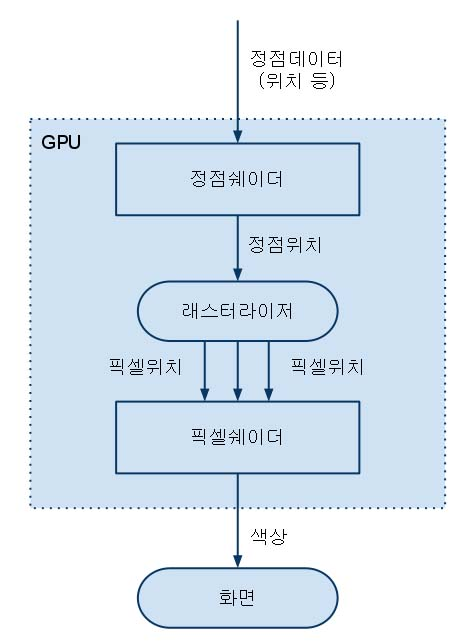
\includegraphics[scale=0.5]{fig1.jpg}
    \caption{극단적으로 간략화시킨 3D 파이프라인}
\end{figure}



그림 1.1에서 정점쉐이더가 입력 값으로 받는 것은 3D 모델 자체입니다. 3D 모델은 폴리곤(polygon, 다각형)으로 구성하는 것이 업계표준인데, 폴리곤이란 결국 삼각형들의 집합에 지나지 않습니다. 삼각형은 3개의 정점(vertex, 꼭짓점이라고도 합니다) 으로 이뤄져 있죠? 그러니 정점데이터가 정점쉐이더의 입력 값이라고 해도 전혀 틀린 게 아니겠네요.

정점쉐이더가 수행하는 가장 중요한 임무는 3D 물체를 구성하는 정점들의 위치를 화면좌표로 변환하는 것입니다. 이를 화가에 비유한다면 투시원근법을 사용하여 실제세계에 있는 물체들을 캔버스 위에 옮겨 그리는 과정이라 할까요? 이렇게 물체의 위치를 다른 공간으로 옮기는 과정을 공간변환(space transformation)이라고 부르는데 이에 대한 자세한 설명은 다음 장에서 드리도록 하겠습니다. 조금 전에 3D 모델은 결국 정점들의 집합이라고 말씀드렸었죠? 따라서 모든 정점을 하나씩 공간 변환하면 3D 물체 자체를 공간 변환하는 것과 똑같은 결과를 얻을 수 있습니다. 이게 바로 정점쉐이더가 하는 일이지요. 그렇다면 정점쉐이더 함수는 몇 번이나 호출될까요? 다음 문장을 보시면 답을 아실 수 있겠네요.

\paragraph{정점쉐이더의 주된 임무는 각 정점의 공간을 변환하는 것이다.}

네, 그렇습니다. 정점쉐이더는 3D 물체를 구성하는 정점의 수만큼 실행됩니다.

정점쉐이더가 반드시 출력하는 결과 값은 화면공간 안에 존재하는 정점의 위치(이외에도 다양한 정보를 정점쉐이더의 결과 값에 담을 수 있습니다. 자세한 내용은 이 책의 뒷부분에서 살펴볼 것입니다.)입니다. 이 위치를 3개씩 그룹 지으면 화면에 출력할 삼각형을 만들 수 있지요.

자, 그렇다면 이 삼각형 안에 픽셀이 몇 개나 들어갈까요? 화면을 구성하는 단위는 픽셀이니까 화면에 뭔가 그림을 그리려면 픽셀을 어디에 몇 개나 그려야 하는지를 알아야겠죠? 이게 바로 래스터라이저(rasterizer)란 장치가 하는 일입니다. 래스터라이저는 정점쉐이더가 출력하는 정점의 위치를 차례대로 3개씩 모아 삼각형을 만든 뒤, 그 안에 들어갈 픽셀들을 찾아냅니다. 자, 그러면 픽셀쉐이더 함수는 몇 번이나 호출될까요? 래스터라이저가 찾아내는 픽셀 수 만큼이겠죠?

그렇다면 위에서 보여드렸던 초 간략 파이프라인의 마지막 단계인 픽셀쉐이더가 하는 일은 무엇일까요? 이미 위에서 살펴본 것 같지만 그래도 다시 한번 반복해 드리지요.

\paragraph{픽셀쉐이더의 주된 임무는 화면에 출력할 최종색상을 계산하는 것이다.}


이제 정점쉐이더와 픽셀쉐이더의 임무를 합치면 아까 제 맘대로 내렸던 쉐이더의 정의가 나오죠?

\paragraph{쉐이더란 화면에 존재하는 각 픽셀의 위치와 색상을 계산하는 함수이다.}


솔직히 이 정도 말씀을 드려도 쉐이더를 처음 접하시는 분들은 아직도 감이 안 잡히실 겁니다. 사실 쉐이더를 짜 보지 않으면 이해가 어렵습니다. 3D 물체를 화면에 그릴 때, 그 물체를 구성하는 픽셀들의 위치와 색을 프로그래머 맘대로 조작하는 거라고 하면 이해가 좀 더 되실까요? 아직도 이해가 안되시더라도 크게 걱정은 마세요 이 책을 읽으시다 보면 '아~ 이런 거였구나~'하고 갑자기 이해가 되실 겁니다. ^^
    
\subsection{쉐이더 프로그래밍}

\href{https://app.box.com/s/9409f61ba4f1a34254c6}{샘플파일 받기}

자, 그럼 쉐이더가 무엇인지는 대충 알아보았는데 쉐이더를 코드를 짠다는 것은 무슨 뜻일까요? 일단 그림 1.1을 다시 한번 살펴보죠. 그림 1.1을 보면 사각형으로 표현한 파이프라인 단계도 있고 둥글게 표현한 것도 있죠? 원형으로 표현한 단계들은 \textbf{GPU(graphics processing unit}, 그래픽 처리장치)가 알아서 처리해주는 -- 즉 프로그래머가 따로 제어할 수 없는 -- 단계들입니다. 그와 반대로 사각형으로 표현한 단계들은 프로그래머가 마음대로 제어할 수 있는 단계들이죠. 이 단계에서 사용할 함수를 작성하는 것이 바로 쉐이더 프로그래밍입니다. 그림 1.1에서 사각형으로 표현된 단계들은 정점쉐이더와 픽셀쉐이더 뿐인 거 보이시죠? 따라서 정점쉐이더와 픽셀쉐이더에 사용할 함수를 하나씩 만드는 것이 쉐이더 프로그래밍입니다. (DirectX 10과 11에서 새로운 쉐이더들이 추가되었습니다. 하지만 아직 실무에서 널리 사용되지 않아서 실용적인 접근이 어렵고, 입문자에게 적당하지 않은 내용이라 이 책에서 다루지 않습니다.)

시중에 나와 있는 여러 쉐이더 언어 중에 이 책에서 사용할 언어는 DirectX에서 지원하는 HLSL입니다. \textbf{HLSL(High Level Shader Language}, 고수준 쉐이더언어)은 C와 매우 비슷한 문법을 사용하는 언어로 \textbf{GLSL}(OpenGL Shader Language의 약자로 OpenGL에서 지원하는 쉐이더 언어입니다. HLSL과 문법 정도가 조금 다릅니다.)이나 \textbf{CgFX}(엔비디아에서 지원하는 쉐이더 언어입니다. HLSL과 한두 개 빼고는 완전히 똑같습니다.)등의 기타 쉐이더 언어와 매우 흡사합니다. 따라서 HLSL을 배우시면 다른 쉐이더 언어를 익히시는데도 큰 무리가 없을 것입니다.

한 언어를 배우는 최선의 방법은 직접 코딩을 하면서 배우는 것입니다. 이 언어의 철학은 이러네, 이 언어의 문법은 저러네 하면서 백날 떠들어봐야 입문자들은 하품만 하고 무슨 이야긴지 알아듣지도 못합니다. 일단 재미있게 코드를 짜봐야 프로그래밍에 애착도 생기고, 애착이 생기면 보다 나은 프로그래머가 되기 위해 노력을 하지요. 따라서 이 책에서는 쓸데없이 HLSL 문법을 나열하면서 독자분들의 짜증을 부추기는 대신 무조건 아주 쉬운 쉐이더부터 짜보는 방법으로 HLSL을 배우도록 하겠습니다. 정 문법이 궁금하신 분들은 부록을 참고하시길 바랍니다.

하지만 HLSL 코드를 곧바로 짜기 전에 준비해야 할 것들이 좀 있군요. 이건 좀 지루하시더라도 꾹 참고 따라 해주시기 바랍니다.

\subsubsection{쉐이더 프로그래밍을 위한 기본준비}

서문에서도 말씀드렸듯이 이 책의 초점은 쉐이더 프로그래밍입니다. 이 책에서 DirectX에 대한 내용을 자세히 다루지 않기로 결정한 이유는 이미 훌륭한 DirectX 입문 책들이 시중에 나와있는데 굳이 DirectX를 다시 처음부터 소개하면서 쓸데없이 지면을 낭비하고 싶지 않았기 때문입니다. (지면이 늘어나면 쓸데없이 책 값도 오릅니다.) 또한 프로그래머 분들 외에 테크니컬 아티스트 분들도 이 책을 읽으실 수 있도록 하기 위해서입니다.

마찬가지 이유로 이 책에서 쉐이더를 만드는 과정도 둘로 나눴습니다. 첫 번째 단계는 쉐이더 작성만을 하는 단계로 AMD(전 ATI) 사의 렌더몽키(render monkey)라는 프로그램을 사용합니다. 이 단계는 프로그래머와 아티스트 분들을 모두 대상으로 하므로 반드시 따라 해 주시기 바랍니다.

두 번째 단계는 렌더몽키에서 만든 쉐이더를 C++/DirectX 프레임워크에서 불러와 사용하는 것으로 프로그래머 분들을 위한 단계입니다. 프로그래머이시더라도 C++/DirectX 프레임워크에 관심이 없으신 분들은 이 단계를 건너 뛰셔도 됩니다. 실제로 쉐이더 코드를 작성하는 곳은 첫 번째 단계입니다.

자, 그러면 위 두 단계에서 쉐이더를 배우는 데 필요한 것들을 준비해보죠.

렌더몽키
렌더몽키는 AMD사에서 제공하는 쉐이더 작성도구로 프로토타이핑에 유용합니다. 부록 디스크에서 /RenderMonkey/ RenderMonkey.2008-12-17-v1.82.322.msi를 찾아 설치해 주세요. 그냥 기본(default) 옵션으로 설치하시면 되겠습니다.

선택사항: 간단한 DirectX 프레임워크
C++/DirectX 프레임워크에서 쉐이더를 실행해보고 싶으신 분들만 이 절을 따라 해주세요.

우선 비주얼 C++ 2008과 DirectX SDK를 설치하시기 바랍니다. 비주얼 C++을 소장하고 계시지 않으신 분들은 마이크로소프트사의 웹 페이지에서 공짜 버전인 익스프레스 버전을 다운받으실 수 있습니다. DirectX SDK는 부록 CD의 DXSDK 폴더에 포함되어 있습니다.

위 두 프로그램의 설치를 마치셨다면 비주얼 C++ 2008에서 부록 CD에 있는 $samples/01_DxFramework/BasicFramework.sln$ 파일을 여시기 바랍니다. 별다른 수정 없이 이 프로그램을 실행하면 다음과 같은 파란 화면을 보실 수 있을 것입니다.


그림 1.2. 별볼일 없는 초 간단 프레임워크


이 프레임워크는 다음과 같은 기능들을 구현합니다.

\begin{itemize}
    \item 창의 생성 및 메시지 루프 등의 기본적인 윈도우 기능
    \item Direct 3D 장치 생성
    \item 텍스처, 모델, 쉐이더 등의 자원 로딩
    \item 간단한 게임루프
    \item 간단한 키보드 입력처리
\end{itemize}

참고로 말씀드리는데 이 프로그램은 쉐이더 코드를 재빨리 실행할 수 있도록 매우 간단하게 만든 프레임워크입니다. 그 결과, 모든 함수들이 .cpp 파일 하나 안에 들어있고, 클래스나 개체도 사용하지 않지요. 따라서 모든 함수들은 C스타일로 작성되어 있고, 모든 변수들도 전역적으로 선언되어 있습니다. \textbf{실제 게임을 만드실 때, 이렇게 프레임워크를 만드시면 절대 안됩니다.} 다시 한 번 말씀드리는데 이 프레임워크는 쉐이더 데모를 실행할 수 있도록 만든 프로그램일 뿐입니다.

자, 그럼 적당히 주의도 드렸으니 이제 프레임워크를 살펴보도록 합시다. 우선 BasicFramework.h를 엽니다.

\begin{lstlisting}[style = CStyle,escapeinside=~~]    
//**********************************************************************
//
// ShaderFramework.h
//
// ~쉐이더 데모를 위한 C스타일의 초간단 프레임워크입니다.~
// ~(실제 게임을 코딩하실 때는 절대 이렇게 프레임워크를~
// ~작성하시면 안됩니다. $-\_-$)~
//
// Author: Pope Kim
//
//**********************************************************************


#pragma once

#include <d3d9.h>
#include <d3dx9.h>

// ---------- ~선언~ ------------------------------------
#define WIN_WIDTH  800
#define WIN_HEIGHT  600

// ---------------- ~함수 프로토타입~ ------------------------

// ~메시지 처리기 관련~
LRESULT WINAPI MsgProc( HWND hWnd, UINT msg, WPARAM wParam, LPARAM lParam );
void ProcessInput(HWND hWnd, WPARAM keyPress);

// ~초기화 과련~
bool InitEverything(HWND hWnd);
bool InitD3D(HWND hWnd);
bool LoadAssets();
LPD3DXEFFECT LoadShader( const char * filename );
LPDIRECT3DTEXTURE9 LoadTexture(const char * filename);
LPD3DXMESH LoadModel(const char * filename);

// ~게임루프 관련~
void PlayDemo();
void Update();

//~렌더링 관련~
void RenderFrame();
void RenderScene();
void RenderInfo();

// ~뒷정리 관련~
void Cleanup();
\end{lstlisting}

% 이 헤더파일에서 눈 여겨 볼만한 것은 WIN_WIDTH와 WIN_HEIGHT밖에 없습니다. 이 두 #define문은 데모 프로그램의 창 크기를 정의합니다. 나머지 코드들은 단순히 함수선언들일 뿐입니다. 실제 함수들의 구현은 ShaderFramework.cpp 파일에 들어 있으니 ShaderFramework.cpp 파일을 열어보도록 할까요?

% 이 파일의 제일 위에는 다음과 같은 전역변수들이 정의되어 있습니다.

% \begin{lstlisting}[style = CStyle]    
% //----------------------------------------------------------------------
% // 전역변수
% //----------------------------------------------------------------------

% // D3D 관련
% LPDIRECT3D9       gpD3D          = NULL;        // D3D
% LPDIRECT3DDEVICE9 gpD3DDevice    = NULL;        // D3D 장치

% // 폰트
% ID3DXFont*        gpFont         = NULL;

% // 모델

% // 쉐이더

% // 텍스처

% // 프로그램 이름
% const char*       gAppName        = "초 간단 쉐이더 데모 프레임워크";
% \end{lstlisting}

% 이제 프로그램의 창을 생성할 차례입니다.
% \begin{lstlisting}[style = CStyle]  
% //-----------------------------------------------------------------------
% // 프로그램 진입점/메시지 루프
% //-----------------------------------------------------------------------

% // 진입점
% INT WINAPI WinMain( HINSTANCE hInst, HINSTANCE, LPSTR, INT )
% {
% \end{lstlisting}
% 프로그램의 창을 생성하려면 우선 윈도우 클래스를 등록해야 합니다.

% \begin{lstlisting}[style = CStyle]  
%     // 윈도우 클래스를 등록한다.
%     WNDCLASSEX wc = { sizeof(WNDCLASSEX), CS_CLASSDC, MsgProc, 0L, 0L,
%                       GetModuleHandle(NULL), NULL, NULL, NULL, NULL,
%                       gAppName, NULL };
%     RegisterClassEx( &wc );


% \end{lstlisting}
% 이제 CreateWindow 함수를 사용해서 위에서 등록한 윈도우 클래스의 인스턴스를 만듭니다. 이 때, 앞서 정의했던 WIN_WIDTH와 WIN_HEIGHT를 창의 크기로 지정합니다.

% \begin{lstlisting}[style = CStyle]  
% // 프로그램 창을 생성한다.
%     DWORD style = WS_OVERLAPPED | WS_CAPTION | WS_SYSMENU | WS_MINIMIZEBOX;
%     HWND hWnd = CreateWindow( gAppName, gAppName,
%                                 style, CW_USEDEFAULT, 0, WIN_WIDTH, WIN_HEIGHT,
%                                 GetDesktopWindow(), NULL, wc.hInstance, NULL );
% \end{lstlisting}

% 창의 크기를 WIN_WIDTH와 WIN_HEIGHT로 만들면 실제 렌더링을 할 수 있는 공간이 이보다 작습니다. 창의 크기에 타이틀 바 및 경계선이 포함되기 때문이라죠. 따라서 실제 렌더링이 가능한 공간(client rect)이 WIN_WIDTH와 WIN_HEIGHT와 같도록 창의 크기를 재조정해야 겠네요.

% \begin{lstlisting}[style = CStyle]  
%     // Client Rect 크기가 WIN_WIDTH, WIN_HEIGHT와 같도록 크기를 조정한다.
%     POINT ptDiff;
%     RECT rcClient, rcWindow;
 
%     GetClientRect(hWnd, &rcClient);
%     GetWindowRect(hWnd, &rcWindow);
%     ptDiff.x = (rcWindow.right - rcWindow.left) - rcClient.right;
%     ptDiff.y = (rcWindow.bottom - rcWindow.top) - rcClient.bottom;
%     MoveWindow(hWnd,rcWindow.left, rcWindow.top, WIN_WIDTH + ptDiff.x, WIN_HEIGHT + ptDiff.y, TRUE);
% \end{lstlisting}
% 이제 창의 크기도 적절히 조정했으니 창을 보여줄 차례입니다.
% \begin{lstlisting}[style = CStyle]  
%     ShowWindow( hWnd, SW_SHOWDEFAULT );
%     UpdateWindow( hWnd );
% \end{lstlisting}

% 다음은 Direct3D를 초기화하고 모든 D3D 자원들(텍스처, 쉐이더, 메쉬 등)을 로딩합니다. 이 모든 기능들은 InitEverything() 함수 안에 포함되어 있습니다. 만약 Direct3D 및 기타 초기화에 실패하면 데모를 보여주는 게 불가능하므로 프로그램을 종료합니다.

% \begin{lstlisting}[style = CStyle]
%     // D3D를 비롯한 모든 것을 초기화한다.
%     if( !InitEverything(hWnd) )
%     {
%         PostQuitMessage(1);
%     }
% \end{lstlisting}
% D3D 및 기타 초기화를 마쳤다면 남은 일은 WM_QUIT 메시지를 받을 때까지 데모를 실행하는 것이 전부입니다. WM_QUIT은 데모를 종료하라는 윈도우 메시지입니다.

% \begin{lstlisting}[style = CStyle]
%     // 메시지 루프
%     MSG msg;
%     ZeroMemory(&msg, sizeof(msg));
%     while(msg.message!=WM_QUIT)
%     {
%         if( PeekMessage( &msg, NULL, 0U, 0U, PM_REMOVE ) )
%         {
%             TranslateMessage( &msg );
%             DispatchMessage( &msg );
%         }
%         else // 메시지가 없으면 게임을 업데이트하고 장면을 그린다
%         {
%             PlayDemo();
%         }
%     }
% \end{lstlisting}
% 데모를 종료할 때가 되면 윈도우 클래스의 등록을 해제하고 프로그램을 끝마칩니다.

% \begin{lstlisting}[style = CStyle]
%     UnregisterClass( gAppName, wc.hInstance );
%     return 0;
% }
% \end{lstlisting}
% 다음은 윈도우 메시지를 처리하는 함수입니다.

% \begin{lstlisting}[style = CStyle]
% // 메시지 처리기
% LRESULT WINAPI MsgProc( HWND hWnd, UINT msg, WPARAM wParam, LPARAM lParam )
% {
%     switch( msg )
%     {
% \end{lstlisting}
% 키보드 입력은 ProcessInput이라는 함수에서 처리할 것입니다.
% \begin{lstlisting}[style = CStyle]
%     case WM_KEYDOWN:
%         ProcessInput(hWnd, wParam);
%         break;
% \end{lstlisting}

% 창이 닫힐 때는 초기화 도중에 생성했던 D3D 자원들을 해제하고 프로그램을 종료하라는 메시지를 보냅니다.

% \begin{lstlisting}[style = CStyle]
%     case WM_DESTROY:
%         Cleanup();
%         PostQuitMessage(0);
%         return 0;
%     }
% \end{lstlisting}
% 이 데모에서 처리하지 않는 윈도우 메시지들은 기본(default) 메시지 처리기가 처리하도록 합니다.

% \begin{lstlisting}[style = CStyle]
%     return DefWindowProc( hWnd, msg, wParam, lParam );
% }
% \end{lstlisting}
% 이 프레임워크가 현재 처리하는 키보드 입력은 ESC 키가 전부입니다. ESC키가 눌리면 프로그램의 실행을 마칩니다.

% \begin{lstlisting}[style = CStyle]
% // 키보드 입력처리
% void ProcessInput( HWND hWnd, WPARAM keyPress)
% {
%  switch(keyPress)
%  {
%  // ESC 키가 눌리면 프로그램을 종료한다.
%  case VK_ESCAPE:
%   PostMessage(hWnd, WM_DESTROY, 0L, 0L);
%   break;
%  }
% }
% \end{lstlisting}

% 이제 초기화 코드를 살펴볼까요?


% \begin{lstlisting}[style = CStyle]
% //------------------------------------------------------------
% // 초기화 코드
% //------------------------------------------------------------
% bool InitEverything(HWND hWnd)
% {

% 우선 InitD3D함수를 호출하여 D3D를 초기화합니다. D3D 초기화에 실패하지 않았다면 LoadAssets() 함수를 통해 모델, 쉐이더, 텍스처 등의 D3D 자원들을 로딩합니다.

%     // D3D를 초기화
%     if( !InitD3D(hWnd) )
%     {
%         return false;
%     }

%     // 모델, 쉐이더, 텍스처 등을 로딩
%     if( !LoadAssets() )
%     {
%         return false;
%     }

% \end{lstlisting}
% 그 다음은 폰트를 로딩할 차례입니다. 이 폰트를 사용하여 화면에 디버그 정보 등을 보여줄 것입니다.

% \begin{lstlisting}[style = CStyle]

%     // 폰트를 로딩
%     if(FAILED(D3DXCreateFont( gpD3DDevice, 20, 10, FW_BOLD, 1, FALSE,
%         DEFAULT_CHARSET, OUT_DEFAULT_PRECIS, DEFAULT_QUALITY,
%         (DEFAULT_PITCH | FF_DONTCARE), "Arial", &gpFont )))
%     {
%  return false;
%     }

%     return true;
% }


% \end{lstlisting}

% 위의 D3DXCreateFont()에서 사용했던 각 매개변수의 의미는 순서대로 다음과 같습니다.

% \begin{itemize}
%     \item gpD3DDevice: D3D 장치
%     \item 20: 폰트의 높이
%     \item 10: 폰트의 너비
%     \item FW_BOLD: 볼드체(두꺼운 폰트)를 이용함
%     \item 1: 밉맵레벨
%     \item FALSE: 이탤릭체를 쓰지 않음
%     \item DEFAULT_CHARSET: 기본 문자셋을 사용
%     \item OUT_DEFAULT_PRECIS: 실제 화면에 출력되는 폰트가 여기서 지정한 속성과 어느 정도 비슷해야 하는지를 설정
%     \item DEFAULT_QUALITY: 여기서 지정하는 폰트와 실제 폰트의 품질이 얼마나 비슷해야 하는지 설정
%     \item DEFAULT_PITCH | FF_DONTCARE: 기본 피치를 사용하고 폰트군은 상관 없음
%     \item "Arial": 사용할 폰트이름
%     \item gpFont: 새로 만든 폰트를 저장할 포인터
% \end{itemize}


% 이제 D3D 객체와 D3D 장치를 생성하는 InitD3D 함수를 살펴봅시다. D3D를 이용해서 자원을 로딩하거나 렌더링을 하려면 반드시 D3D장치를 생성해야 합니다.


% \begin{lstlisting}[style = CStyle]

% // D3D 객체 및 장치 초기화
% bool InitD3D(HWND hWnd)
% {
% \end{lstlisting}


% \begin{lstlisting}[style = CStyle]
% 우선 Direct3D 객체를 구합니다.

%     // D3D 객체
%     gpD3D = Direct3DCreate9( D3D_SDK_VERSION ); 
%     if ( !gpD3D )
%     {
%         return false;
%     }
% \end{lstlisting}

% 그 다음에는 D3D 장치를 생성할 때 필요한 구조체에 정보를 채워 넣겠습니다.

% \begin{lstlisting}[style = CStyle]
%     // D3D장치를 생성하는데 필요한 구조체를 채워 넣는다.
%     D3DPRESENT_PARAMETERS d3dpp;
%     ZeroMemory( &d3dpp, sizeof(d3dpp) );

%     d3dpp.BackBufferWidth            = WIN_WIDTH;
%     d3dpp.BackBufferHeight           = WIN_HEIGHT;
%     d3dpp.BackBufferFormat           = D3DFMT_X8R8G8B8;
%     d3dpp.BackBufferCount            = 1;
%     d3dpp.MultiSampleType            = D3DMULTISAMPLE_NONE;
%     d3dpp.MultiSampleQuality         = 0;
%     d3dpp.SwapEffect                 = D3DSWAPEFFECT_DISCARD;
%     d3dpp.hDeviceWindow              = hWnd;
%     d3dpp.Windowed                   = TRUE;
%     d3dpp.EnableAutoDepthStencil     = TRUE;
%     d3dpp.AutoDepthStencilFormat     = D3DFMT_D24X8;
%     d3dpp.Flags                      = D3DPRESENTFLAG_DISCARD_DEPTHSTENCIL;
%     d3dpp.FullScreen_RefreshRateInHz = 0;
%     d3dpp.PresentationInterval       = D3DPRESENT_INTERVAL_ONE;

% \end{lstlisting}

% 위에서 주목할만한 정보들은 다음과 같습니다.

% \begin{itemize}
%     \item BackBufferWidth: 백버퍼(렌더링 영역)의 너비
%     \item BackBuferHeight: 백버퍼의 높이
%     \item BackBufferFormat: 백버퍼의 포맷
%     \item AutoDepthStencilFormat: 깊이/스텐실 버퍼의 포맷
%     \item SwapEffect: 백버퍼를 스왑(swap)할 때의 효과. 성능 상 D3DSWAPEFFECT_DISCARD를 사용하는 것이 좋습니다.
%     \item PresentationInterval: 모니터 주사율과 백버퍼를 스왑하는 빈도간의 관계. 
%     \item D3DPRESENT_INTERVAL_ONE은 모니터가 수직동기될 때마다 백버퍼를 스왑해 줍니다. 게임에서는 성능상 모니터의 수직동기를 기다리지 않고 곧바로 스왑해 주는 경우가 많습니다.(D3DPRESENT IMMEDIATE). 단, 이럴 땐 전 프레임과 현재 프레임이 서로 찢겨 보이는 부작용이 있습니다.
% \end{itemize}




% 이제 위에서 채워 넣은 정보들을 이용해서 D3D장치를 생성합니다.

% \begin{lstlisting}[style = CStyle]
%     // D3D장치를 생성한다.
%     if( FAILED( gpD3D->CreateDevice( D3DADAPTER_DEFAULT, D3DDEVTYPE_HAL, hWnd,
%         D3DCREATE_HARDWARE_VERTEXPROCESSING,
%         &d3dpp, &gpD3DDevice ) ) )
%     {
%         return false;
%     }

%     return true;
% }
% \end{lstlisting}

% D3D 자원을 읽어오는 LoadAssets() 함수 안에는 현재 아무 내용도 들어있지 않습니다. 이 책을 진행하면서 텍스처, 쉐이더, 모델 등을 읽어올 일이 있을 때마다 이 함수 안에서 LoadShader(), LoadTexture(), LoadModel() 함수들을 호출하겠습니다.

% bool LoadAssets()
% {
%     // 텍스처 로딩

%     // 쉐이더 로딩

%     // 모델 로딩

%     return true;
% }

% 다음은 .fx 포맷으로 저장된 쉐이더 파일을 불러오는 LoadShader() 함수입니다. .fx파일은 정점쉐이더와 픽셀쉐이더를 모두 포함하고 있는 텍스트 파일로 D3DXCreateEffectFromFile() 함수를 통해 로딩 및 컴파일합니다. 따라서 HLSL코드에 문법적인 오류가 있다면 이 함수를 호출하는 도중에 쉐이더 컴파일 에러가 나겠죠? 그럴 때는 D3DXCreateEffectFromFile()의 마지막 매개변수를 통해 에러메시지를 구해올 수 있습니다. 이 에러메시지를 비주얼 C++의 출력 창에 보여주도록 하겠습니다.


% // 쉐이더 로딩
% LPD3DXEFFECT LoadShader(const char * filename )
% {
%     LPD3DXEFFECT ret = NULL;
%     LPD3DXBUFFER pError = NULL;
%     DWORD dwShaderFlags = 0;

% #if _DEBUG
%     dwShaderFlags |= D3DXSHADER_DEBUG;
% #endif

%     D3DXCreateEffectFromFile(gpD3DDevice, filename,
%         NULL, NULL, dwShaderFlags, NULL, &ret, &pError);

%     // 쉐이더 로딩에 실패한 경우 output창에 쉐이더
%     // 컴파일 에러를 출력한다.
%     if(!ret && pError)
%     {
%         int size  = pError->GetBufferSize();
%         void *ack = pError->GetBufferPointer();

%         if(ack)
%         {
%             char* str = new char[size];
%             sprintf(str, (const char*)ack, size);
%             OutputDebugString(str);
%             delete [] str;
%         }
%     }

%     return ret;
% }

% 위에서 D3DXCreateEffectFromFile() 함수를 호출할 때 사용한 인자들의 의미는 순서대로 아래와 같습니다.

% gpD3DDevice: D3D 장치
% filename: 읽어올 쉐이더 파일의 이름
% NULL: 쉐이더를 컴파일 할 때 추가로 사용할 #define 정의
% NULL: #include 지시문을 처리할 때 사용할 인터페이스 포인터
% dwShaderFlags: 쉐이더를 컴파일 할 때 사용할 플래그
% NULL: 매개변수 공유에 사용할 이펙트 풀
% ret: 로딩된 이펙트를 저장할 포인터
% pError: 컴파일러 에러 메시지를 가리킬 포인터


% 다음은 .x 포맷으로 저장된 모델을 로딩해오는 코드입니다. .x 파일은 DirectX에서 자체적으로 지원하는 메쉬 포맷입니다.

% // 모델 로딩
% LPD3DXMESH LoadModel(const char * filename)
% {
%     LPD3DXMESH ret = NULL;
%     if ( FAILED(D3DXLoadMeshFromX(filename,D3DXMESH_SYSTEMMEM, gpD3DDevice,
%         NULL,NULL,NULL,NULL, &ret)) )
%     {
%         OutputDebugString("모델 로딩 실패: ");
%         OutputDebugString(filename);
%         OutputDebugString("\n");
%     };

%     return ret;
% }

% 위에서 D3DXLoadMeshFromX() 호출에 사용했던 매개변수의 의미는 순서대로 다음과 같습니다.

% filename: 로딩해 올 메쉬의 파일명
% D3DXMESH_SYSTEMMEM: 시스템 메모리에 메쉬를 로딩할 것
% gpD3DDevice: D3D 장치
% NULL: 인접 삼각형 데이터를 따로 구해오지 않음.
% NULL: 머테리얼(material) 정보를 따로 구해오지 않음
% NULL: 이펙트 인스턴스를 따로 구해오지 않음
% NULL: 머테리얼 수를 따로 구해오지 않음
% ret: 로딩해온 메쉬를 저장할 포인터


% 아래는 다양한 포맷으로 저장된 이미지들을 텍스처로 로딩해 오는 LoadTexture() 함수입니다.

% // 텍스처 로딩
% LPDIRECT3DTEXTURE9 LoadTexture(const char * filename)
% {
%     LPDIRECT3DTEXTURE9 ret = NULL;
%     if ( FAILED(D3DXCreateTextureFromFile(gpD3DDevice, filename, &ret)) )
%     {
%         OutputDebugString("텍스처 로딩 실패: ");
%         OutputDebugString(filename);
%         OutputDebugString("\n");
%     }

%     return ret;
% }


% 다음은 게임루프 함수인 PlayDemo()입니다. 이 함수는 처리할 윈도우 메시지가 없을 때마다 호출됩니다. 실제 게임에서는 지난 프레임으로부터 경과한 시간을 구해서 업데이트 및 렌더링에 사용할 테지만 이 프레임워크에서는 간략함을 위해 그 부분을 생략했습니다.


% //------------------------------------------------------------
% // 게임루프
% //------------------------------------------------------------
% void PlayDemo()
% {
%     Update();
%     RenderFrame();
% }

% 현재 Update() 함수에는 아무 내용도 없습니다. 나중에 필요하다면 코드를 채워 넣도록 하지요.


% // 게임로직 업데이트
% void Update()
% {
% }

% 다음은 정작 무언가를 그리는 함수인 RenderFrame()입니다.

% //------------------------------------------------------------
% // 렌더링
% //------------------------------------------------------------

% void RenderFrame()
% {

% 우선 화면을 파란색으로 지웁니다.

%     D3DCOLOR bgColour = 0xFF0000FF; // 배경색상 - 파랑

%     gpD3DDevice->Clear( 0, NULL, (D3DCLEAR_TARGET | D3DCLEAR_ZBUFFER),
%         bgColour, 1.0f, 0 );

% 그 후, 장면(scene)과 디버그 정보를 그립니다.

%     gpD3DDevice->BeginScene();
%     {
%         RenderScene();  // 3D 물체등을 그린다.
%         RenderInfo();  // 디버그 정보 등을 출력한다.
%     }
%     gpD3DDevice->EndScene();


% 모든 그리기를 마쳤다면 백 버퍼에 저장되어 있는 렌더링 결과를 화면에 뿌려줍니다.

%     gpD3DDevice->Present( NULL, NULL, NULL, NULL );
% }


% 현재 3D 물체 등을 그리는 RenderScene() 함수에는 아무 코드도 들어있지 않습니다. 다음 장에서 3D 물체를 그릴 때 여기에 코드를 채워 넣도록 하지요.

% // 3D 물체 등을 그린다.
% void RenderScene()
% {
% }

% RenderInfo() 함수는 간단한 키 매핑 정보를 화면에 보여줍니다.

% // 디버그 정보 등을 출력.
% void RenderInfo()
% {
%     // 텍스트 색상
%     D3DCOLOR fontColor = D3DCOLOR_ARGB(255,255,255,255);  

%     // 텍스트를 출력할 위치
%     RECT rct;
%     rct.left=5;
%     rct.right=WIN_WIDTH / 3;
%     rct.top=5;
%     rct.bottom = WIN_HEIGHT / 3;
 
%     // 키 입력 정보를 출력
%     gpFont->DrawText(NULL, "데모 프레임워크\n\nESC: 데모종료", -1, &rct,
%         0, fontColor );
% }

% 프로그램을 종료할 때, GPU상의 메모리 누수를 방지하려면 D3D를 통해 생성했던 자원들을 모두 해제(release)해줘야 합니다. 자원들을 모두 해제한 뒤에는 D3D 장치와 D3D 객체들도 해제해 줍니다.

% //------------------------------------------------------------
% // 뒷정리 코드.
% //------------------------------------------------------------

% void Cleanup()
% {
%     // 폰트를 release 한다.
%     if(gpFont)
%     {
%         gpFont->Release();
%         gpFont = NULL;
%     }

%     // 모델을 release 한다.

%     // 쉐이더를 release 한다.

%     // 텍스처를 release 한다.

%     // D3D를 release 한다.
%     if(gpD3DDevice)
%     {
%         gpD3DDevice->Release();
%         gpD3DDevice = NULL;
%     }

%     if(gpD3D)
%     {
%         gpD3D->Release();
%         gpD3D = NULL;
%     }
% }


% 자, 이것으로 아주 간단한 쉐이더 프레임워크의 작성을 마쳤습니다. 위의 코드가 잘 이해가 안 되시는 분들이 계실지도 모르겠는데, 이 책에서 HLSL 프로그래밍을 익히는 데는 크게 문제가 안됩니다. 단, 그래픽 프로그래머가 되는 것이 꿈이신 분들은 이 책을 마친 뒤에라도 반드시 DirectX를 제대로 배우시라고 권해드리고 싶습니다.

% 여기까지 다소 지루한 준비과정을 견뎌내시느라 수고하셨습니다. 후딱 정리를 마친 뒤에 다음 장부터 실제로 재미있게 쉐이더를 작성해 보기로 하죠!

% 정리
% 다음은 이 장에서 배운 내용을 짧게 요약해 놓은 것입니다.
% \begin{itemize}
%     \item 쉐이더는 어느 픽셀을 어떤 색으로 칠할지를 계산하는 함수이다.
%     \item 쉐이더를 화가가 그림을 그리는 것에 비유하면 정점쉐이더는 투시를 픽셀쉐이더는 명암을 담당한다.
%     \item 쉐이더 프로그래밍이란 정점쉐이더와 픽셀쉐이더에서 실행시킬 함수를 작성하는 것이다.
%     \item AMD사의 렌더몽키를 사용하면 재빨리 쉐이더를 프로토타입할 수 있다.
% \end{itemize}

\end{document}